\documentclass[a4paper,11pt]{beamer}

\mode<presentation> {

% The Beamer class comes with a number of default slide themes
% which change the colors and layouts of slides. Below this is a list
% of all the themes, uncomment each in turn to see what they look like.

%\usetheme{default}
%\usetheme{AnnArbor}
%\usetheme{Antibes}
%\usetheme{Bergen}
%\usetheme{Berkeley}
%\usetheme{Berlin}
%\usetheme{Boadilla}
%\usetheme{CambridgeUS}
%\usetheme{Copenhagen}
%\usetheme{Darmstadt}
%\usetheme{Dresden}
%\usetheme{Frankfurt}
%\usetheme{Goettingen}
%\usetheme{Hannover}
%\usetheme{Ilmenau}
%\usetheme{JuanLesPins}
%\usetheme{Luebeck}
%\usetheme{Madrid}
%\usetheme{Malmoe}
%\usetheme{Marburg}
%\usetheme{Montpellier}
%\usetheme{PaloAlto}
\usetheme{Pittsburgh}
%\usetheme{Rochester}
%\usetheme{Singapore}
%\usetheme{Szeged}
%\usetheme{Warsaw}

% As well as themes, the Beamer class has a number of color themes
% for any slide theme. Uncomment each of these in turn to see how it
% changes the colors of your current slide theme.

%\usecolortheme{albatross}
%\usecolortheme{beaver}
%\usecolortheme{beetle}
%\usecolortheme{crane}
\usecolortheme{dolphin}
%\usecolortheme{dove}
%\usecolortheme{fly}
%\usecolortheme{lily}
%\usecolortheme{orchid}
%\usecolortheme{rose}
%\usecolortheme{seagull}
%\usecolortheme{seahorse}
%\usecolortheme{whale}
%\usecolortheme{wolverine}

%\setbeamertemplate{footline} % To remove the footer line in all slides uncomment this line
%\setbeamertemplate{footline}[page number] % To replace the footer line in all slides with a simple slide count uncomment this line

%\setbeamertemplate{navigation symbols}{} % To remove the navigation symbols from the bottom of all slides uncomment this line
}
\usepackage{color, colortbl}
\usepackage[absolute,overlay]{textpos}
%----------------------------
\usepackage[utf8]{inputenc}
\usepackage[spanish]{babel}
\usepackage[T1]{fontenc}
%----------------------------
\usepackage{graphicx}
\usepackage{booktabs}
\usepackage{multirow}
\usepackage{amsthm}
\usepackage{amsmath}
\usepackage{pifont}
\makeatletter
\newcommand*{\bdiv}{%
  \nonscript\mskip-\medmuskip\mkern5mu%
  \mathbin{\operator@font div}\penalty900\mkern5mu%
  \nonscript\mskip-\medmuskip
}
\makeatother

\uselanguage{spanish}
\deftranslation[to=spanish]{Theorem}{Teorema}
\deftranslation[to=spanish]{theorem}{teorema}
\deftranslation[to=spanish]{Lemma}{Lema}
\deftranslation[to=spanish]{lemma}{lema}
\deftranslation[to=spanish]{Definition}{Definición}

\newcounter{saveenumi}
\newcommand{\seti}{\setcounter{saveenumi}{\value{enumi}}}
\newcommand{\conti}{\setcounter{enumi}{\value{saveenumi}}}
\newcommand{\specialcell}[2][c]{%
  \begin{tabular}[#1]{@{}r@{}}#2\end{tabular}}

\newcommand{\cmark}{\ding{51}}%
\newcommand{\xmark}{\ding{55}}%
\newcommand{\plusmark}{\ding{70}}

\usepackage{listings}
% \usepackage[toc]{glossaries} %xindy
% \makeglossaries
%----------------------------
\graphicspath{{imgs/}}

\definecolor{ashgrey}{rgb}{0.7, 0.75, 0.71}

\title[ISDB-Tb Extendido]{Integración de servicios audiovisuales de TV terrestre e IPTV} % The short title appears at the bottom of every slide, the full title is only on the title page

\author{Santiago Seifert} % Your name
\institute[UNLP] % Your institution as it will appear on the bottom of every slide, may be shorthand to save space
{
Universidad Nacional de La Plata \\ % Your institution for the title page
\medskip
\textit{santiagoseifert@gmail.com} % Your email address
}
\date{7 de Septiembre de 2015}

\begin{document}

\begin{frame}
\titlepage % Print the title page as the first slide
\end{frame}

% \begin{frame}
% \frametitle{Contenidos de la presentación} % Table of contents slide, comment this block out to remove it
% \tableofcontents % Throughout your presentation, if you choose to use \section{} and \subsection{} commands, these will automatically be printed on this slide as an overview of your presentation
% \end{frame}

% %----------------------------------------------------------------------------------------
% %  & PRESENTATION SLIDES
% %----------------------------------------------------------------------------------------

% %------------------------------------------------
% \section{First Section} % Sections can be created in order to organize your presentation into discrete blocks, all sections and subsections are automatically printed in the table of contents as an overview of the talk
% %------------------------------------------------

% \subsection{Subsection Example} % A subsection can be created just before a set of slides with a common theme to further break down your presentation into chunks


%------------------------------------------------
% TEMARIO.

% TODO:
% \begin{frame}
% 	\frametitle{Temario}
% 	\tableofcontents[sections={1}]
% \end{frame}

% \begin{frame}
% 	\frametitle{Temario}
% 	\tableofcontents[sections={2}]
% \end{frame}

% \begin{frame}
% 	\frametitle{Temario}
% 	\tableofcontents[sections={3}]
% \end{frame}

% \begin{frame}
% 	\frametitle{Temario}
% 	\tableofcontents[sections={4}]
% \end{frame}

% \begin{frame}
% 	\frametitle{Temario}
% 	\tableofcontents[sections={5}]
% \end{frame}

% \begin{frame}
% \frametitle{Temario}
% \begin{center}
% \begin{itemize}
% \item Introducción
% 	\begin{itemize}
% 		\item Motivación
% 		\item Hipótesis
% 		\item Objetivos
% 	\end{itemize}
% \item Introducción Técnica
% 	\begin{itemize}
% 		\item Conceptos útiles
% 		\item ISDB-Tb
% 		\item Generación de contenidos en ISDB-Tb
% 		\begin{itemize}
% 			\item OpenCaster
% 		\end{itemize}
% 		\item Recepción y decodificación de contenidos en ISDB-Tb
% 		\begin{itemize}
% 			\item Reproductor de TV Digital \textbf{Wari}
% 		\end{itemize}
% 		\item IPTV
% 	\end{itemize}
% \item Diseño y desarrollo
% 	\begin{itemize}
% 		\item Señalización
% 			\begin{itemize}
% 				\item Elementary Streams Relocation Descriptor
% 			\end{itemize}
% 		\item Construcción del Flujo de Transporte de referencia
% 			\begin{itemize}
% 				\item Extensión de OpenCaster
% 				\item Aumento de un Flujo de Transporte existente
% 			\end{itemize}
% 		\item Emisión de IPTV
% 		\item Recepción de Contenidos
% 			\begin{itemize}
% 				\item Reproductor de TV Híbrida \textbf{Mara}
% 			\end{itemize}
% 	\end{itemize}
% \item Evaluación
% 	\begin{itemize}
% 		\item Infraestructura
% 			\begin{itemize}
% 				\item Escenario Real
% 				\item Escenario de prueba
% 			\end{itemize}
% 		\item Análisis General
% 			\begin{itemize}
% 				\item Número de Servicios
% 				\item Flujos Elementales Múltiples
% 				\item Guía electrónica de programación
% 				\item \emph{Closed Caption}
% 				\item Gestión de Audiencias
% 				\item Aplicaciones Interactivas
% 				\item Tiempos de sintonización
% 			\end{itemize}
% 	\end{itemize}
% \item Conclusión
% 	\begin{itemize}
% 		\item Características del resultado
% 		\item Mara
% 		\item Trabajo Futuro
% 		\begin{itemize}
% 			\item Reubicación en \emph{Object Based Broadcasting}
% 			\item Reubicación por eventos
% 			\item Soporte de IPV6
% 			\item Omisión de PMT pequeñas
% 		\end{itemize}
% 		\item Conclusión
% 	\end{itemize}
% \end{itemize}

% \end{center}
% \end{frame}



\section{Introducción}

\begin{frame}
%\frametitle{A first slide}

\begin{center}
\Huge Introducción
\end{center}

\end{frame}
	% \begin{frame}
	% 	\frametitle{Introducción}
		
	% \end{frame}

	\subsection{Motivación}
		\begin{frame}
			\frametitle{Motivación}
			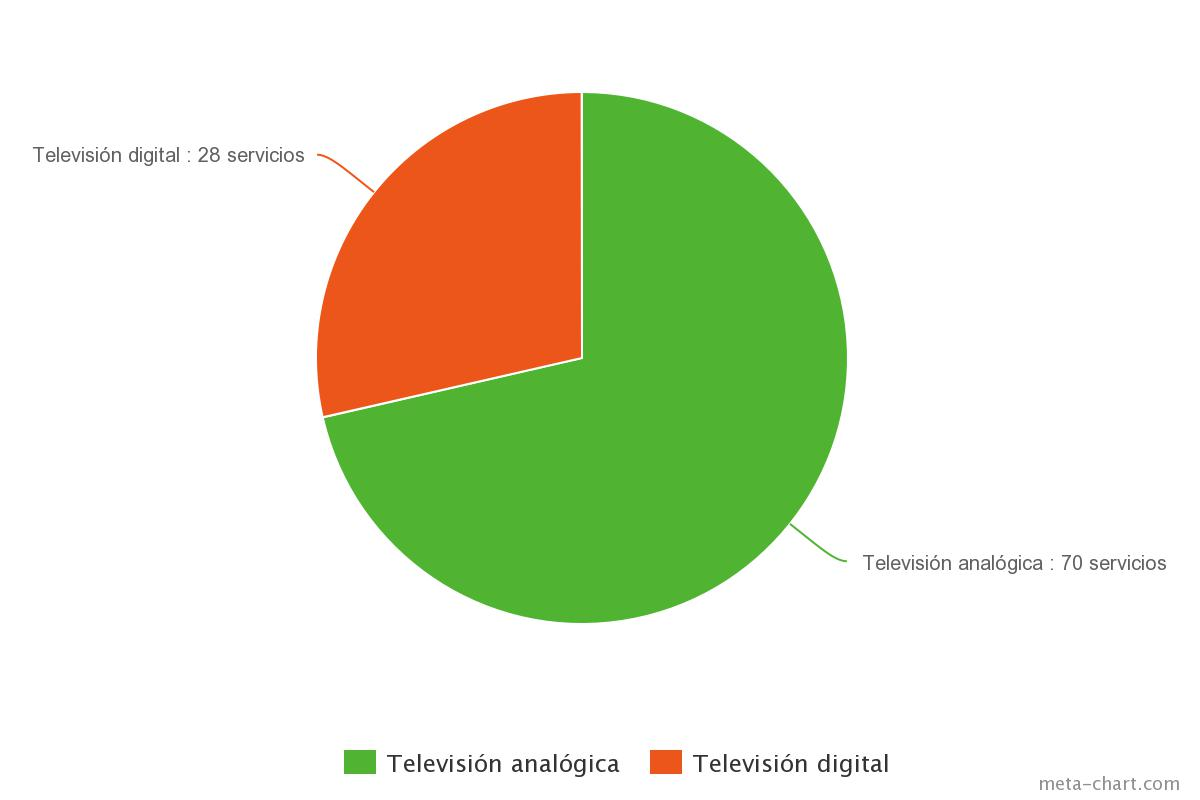
\includegraphics[height=6.5cm]{numero_servicios_vs.jpeg}
		\end{frame}

		\begin{frame}
			\frametitle{Motivación}
			\begin{center}
			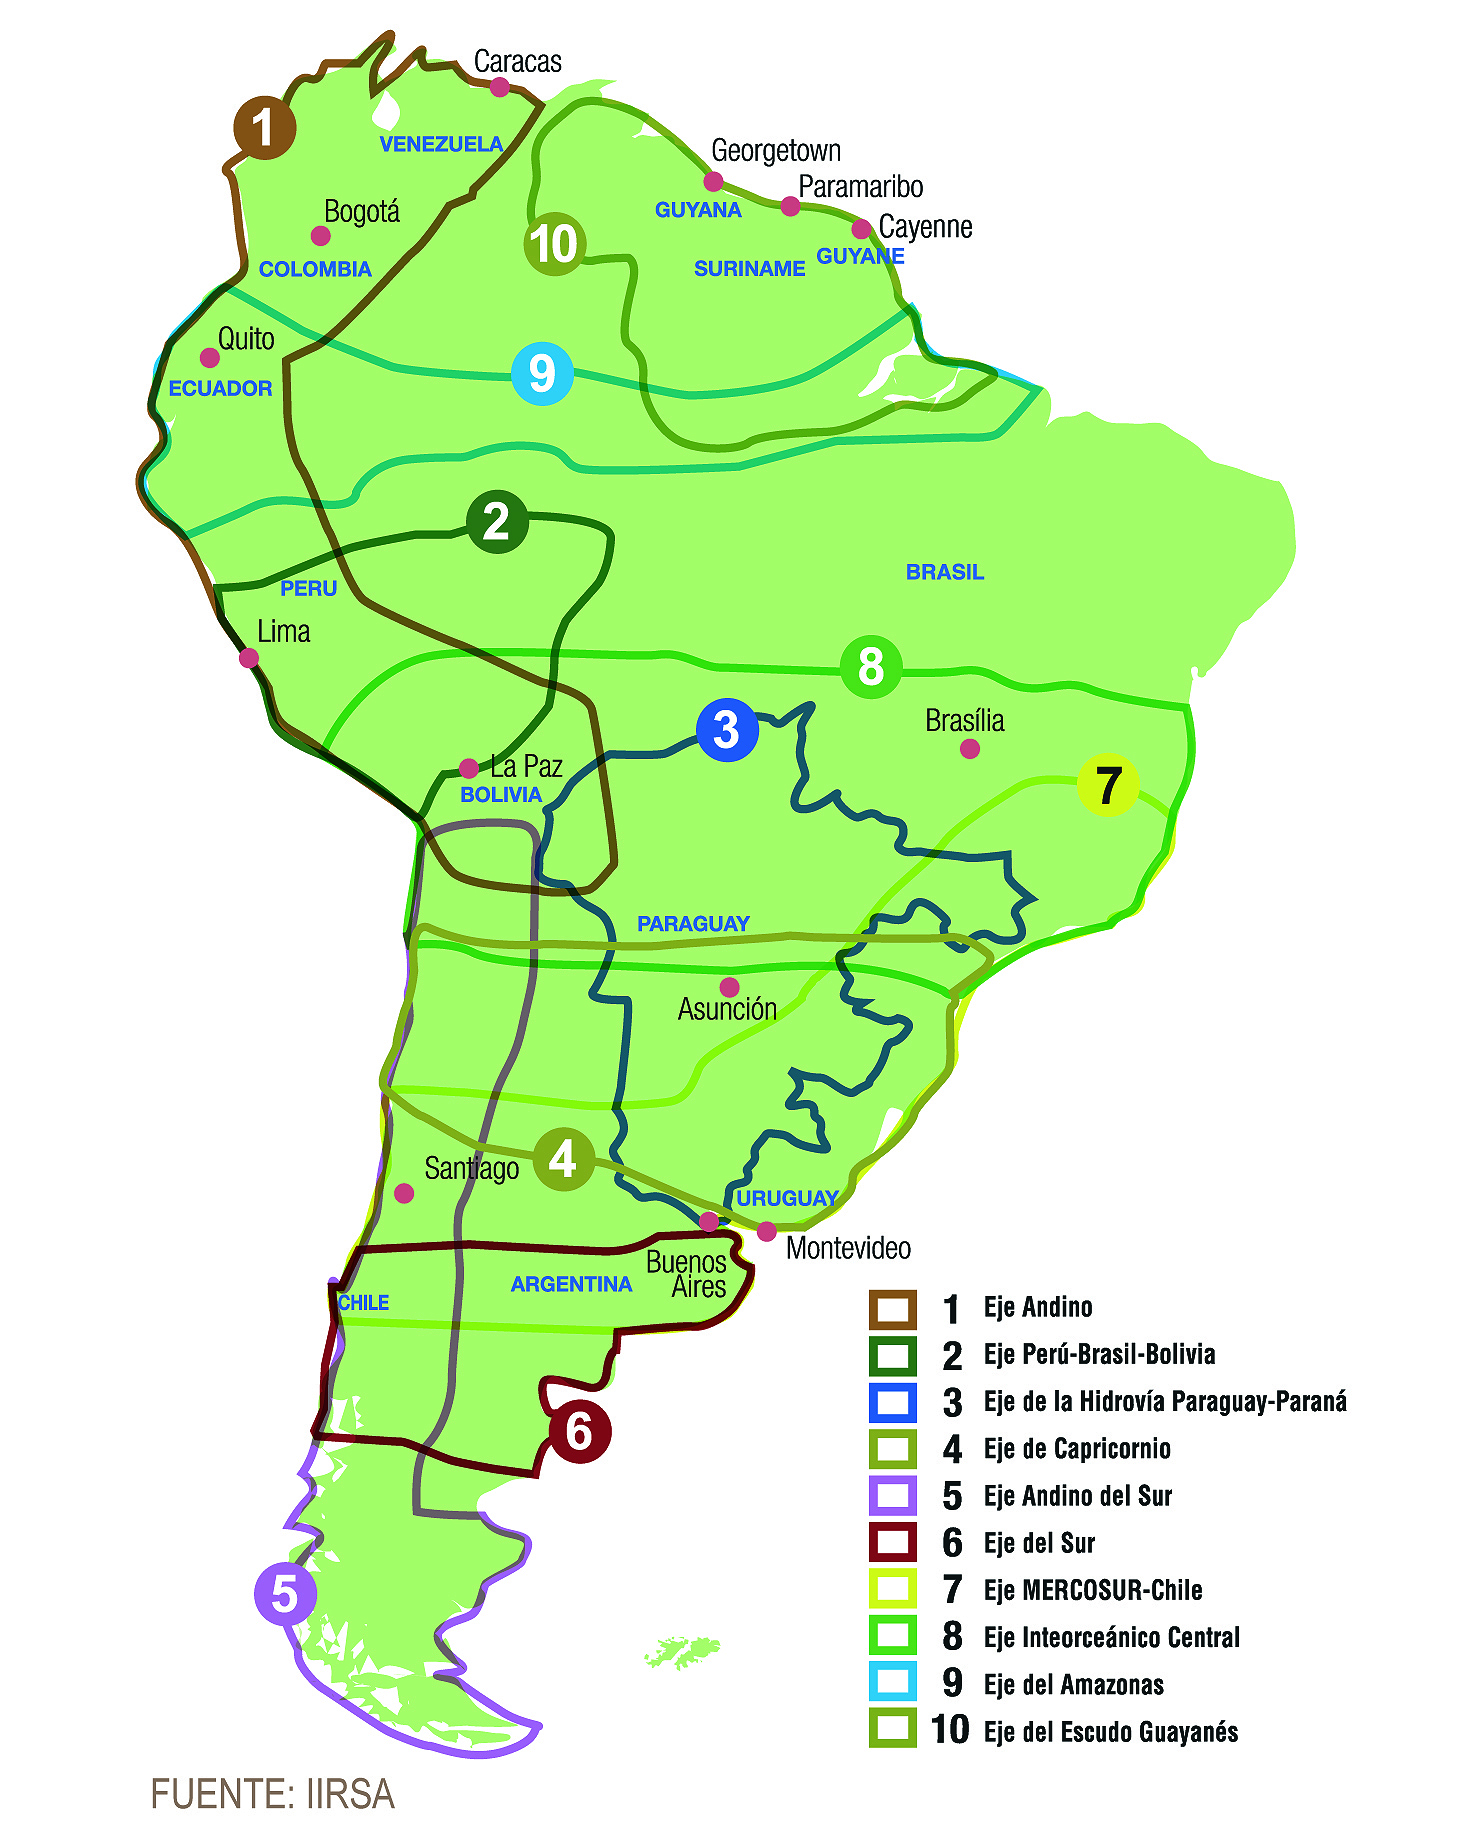
\includegraphics[height=7.3cm]{unasur.jpg}
			\end{center}
		\end{frame}

		\begin{frame}
			\frametitle{Motivación}
			\begin{center}
			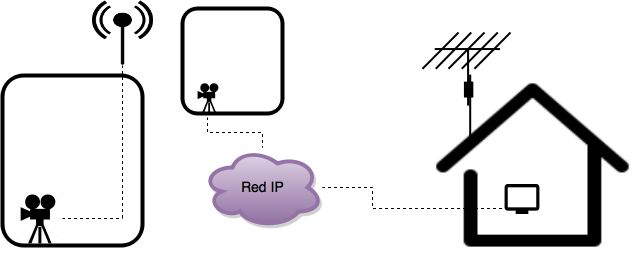
\includegraphics[height=3cm]{isdbt_con_ip.png}
			\end{center}

			% Ref penales
		\end{frame}

	\subsection{Hipótesis}
		\begin{frame}
			\frametitle{Hipótesis}
			\begin{itemize}
				\item Mitigar la limitación del tamaño de la lista de servicios
				\item Combinar ISDB-Tb con IPTV
				\item Conservar ancho de banda efectivo de RF
			\end{itemize}
		\end{frame}

	\subsection{Objetivos}
		\begin{frame}
			\frametitle{Objetivos}
			\begin{itemize}	
				\item Retrocompatibilidad
				\item Minimización de cambios
				\item Aprovechamiento eficiente de la infraestructura
				\item Transparencia para el usuario
			\end{itemize}
		\end{frame}

\section{Introducción Técnica}
\begin{frame}
%\frametitle{A first slide}

\begin{center}
\Huge Introducción Técnica
\end{center}

\end{frame}

	\begin{frame}
		\frametitle{Introducción Técnica}
		\begin{center}
			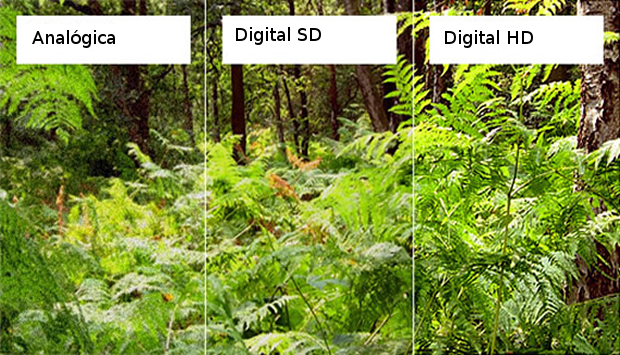
\includegraphics[height=4cm]{analog_vs_digital_sd_hd.jpg} 
		\end{center}
	\end{frame}

	\subsection{Conceptos preliminares}
		\begin{frame}
			\frametitle{Conceptos preliminares: TV Digital}
% \begin{columns}[c,t] % The "c" option specifies centered vertical alignment while the "t" option is used for top vertical alignment

% \column{.45\textwidth} % Left column and width
% \textbf{ISDB-T}
% \begin{enumerate}
% \item Robusto
% \item Limitación de servicios
% \item Infraestructura simple
% \end{enumerate}

% \column{.45\textwidth} % Right column and width
% \textbf{IPTV}
% \begin{enumerate}
% \item Suceptible a sobreexigencia
% \item Lista de servicios potencialmente grande
% \item Infraestructura compleja
% \end{enumerate}
% \end{columns}

			\begin{columns}[c] % ,t
				\column{.45\textwidth}
					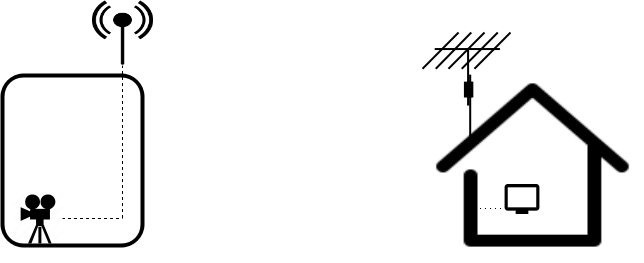
\includegraphics[width=5cm]{terrestre.png}
				\column{.45\textwidth}
					\begin{itemize}
						\item Mejor calidad
						\item Permite alta definición
						\item Permite multiprogramación
						\item Permite múltiples flujos elementales
						\item Permite servicios complementarios
						\item Ahorra ancho de banda
						\item Permite multiplicidad de dispositivos
					\end{itemize}
			\end{columns}
		\end{frame}

		\begin{frame}
			\frametitle{Conceptos preliminares: Tipos de emisión}
			\begin{itemize}
				\item Terrestre(ATSC, DVB, DTMB, ISDB-Tb)
				\item Satelital
				\item Cable
				\item Over the Top
				\item IPTV
			\end{itemize}
		\end{frame}

		\begin{frame}
			\frametitle{Conceptos preliminares: IPTV}
			\begin{definition}
				Define la entrega de servicios (televisión, video, audio, texto, imágenes, datos) sobre redes basadas en IP manejadas para proveer el nivel requerido de calidad de servicio y experiencia, seguridad, interactividad y confiabilidad.
			\end{definition}

		\end{frame}


	\subsection{ISDB-Tb}
		\begin{frame}
			\frametitle{ISDB-Tb}
			\begin{center}
				\includegraphics[width=11cm]{isdbt_en_el_mundo.png}
			\end{center}
		\end{frame}

		\begin{frame}
			\frametitle{ISDB-Tb}
			\begin{center}
				\includegraphics[width=11cm]{bandas_uhf.png}
			\end{center}
		\end{frame}

		\subsubsection{Modualción y bitrate disponible}
		\begin{frame}
			\frametitle{Modulación y Bitrate disponible}
			\begin{center}
				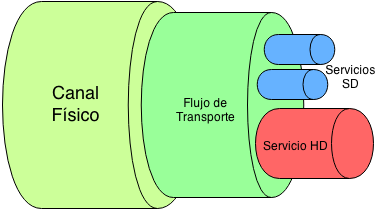
\includegraphics[width=7.5cm]{canal_fisico.png}
			\end{center}			
		\end{frame}

		\begin{frame}
			\frametitle{Modulación y Bitrate disponible}
			\begin{table}
			\begin{center}
			\resizebox{\linewidth}{!}{
				\begin{tabular}{| l | c | c | c |}
				\hline 
				\textbf{Nombre del servicio} & \textbf{Tipo de video} & \textbf{\begin{tabular}[x]{@{}c@{}}Bitrate promedio\\utilizado\end{tabular}} & \textbf{\begin{tabular}[x]{@{}c@{}}Porcentaje del bitrate\\del flujo utilizado\end{tabular}}\\
				\hline 
				TV Pública HD & \emph{High Definition Video} & 11,7 Mbps & 67,7\% \\
				\hline
				TV Pública & \emph{Low Definition Video} & 0,3 Mbps & 1,9\% \\
				\hline
				Tecnópolis & \emph{Standard Definition Video} & 2,0 Mpbs & 11,7\% \\
				\hline
				\hline
				\textbf{Total:} & --- & 14 Mbps & 81,3\% \\
				\hline 
				\end{tabular}
			}
			\caption{Utilización de bitrate por el video en el ejemplo de Canal 23\label{tab:avgbitrates}}
			\end{center}
			\end{table}
		\end{frame}

		\subsubsection{MPEG-2 Transport Stream}
		\begin{frame}
			\frametitle{MPEG-2 Transport Stream}
			\begin{itemize}
				\item Da significado a los bytes modulados
				\item Diseñado para ambientes no confiables
		 		\item Multiplexación de servicios con bitrates variables e independientes
		 		\item Provee mecanismos para la sincronización de flujos de audio y video
		 		\item Es un formato extensible
		 	\end{itemize}
		\end{frame}

		% \begin{frame}
		% 	\frametitle{Características de MPEG-2 Transport Stream}
		% 		\begin{itemize}
					
		%  		\end{itemize}
		% \end{frame}

			\begin{frame}
				\frametitle{Estructura de paquetes MPEG-TS}
				\begin{center}
					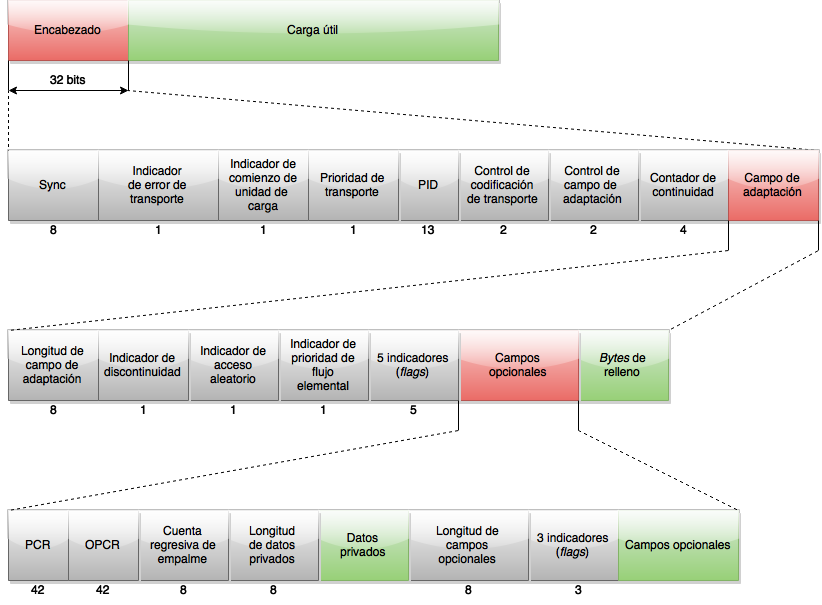
\includegraphics[width=7.5cm]{appendix_ts_packet_detail.png}
				\end{center}
			\end{frame}

			\begin{frame}
				\frametitle{Recepción de señal ISDB-Tb}
				\begin{tabular}[t]{ | c | c | c | c | }
			\hline
			Canal 	& Servicio 		& Logotipo		&		Formato de video \\
			\hline\hline
			\multirow{5}{*}{22 (521MHz)}	& Encuentro 	& 
\includegraphics[width=1cm]{logoencuentro.png}	& SD (576i, 50Hz) \\\cline{2-4}
								& Paka Paka 	& 
\includegraphics[width=1cm]{logopakapaka.png}	& SD (576i, 50Hz) \\\cline{2-4}
								& TaTeTi 		& 
\includegraphics[width=1cm]{logotateti.png}	& SD (576i, 50Hz) \\\cline{2-4}
								& INCAA TV 		& 
\includegraphics[width=1cm]{logoincaa.png}	& SD (576i, 50Hz) \\\cline{2-4}
								& Encuentro LD 	& 
\includegraphics[width=1cm]{logoencuentro.png}	& LD (240p, 30Hz) \\\hline\hline
			\multirow{3}{*}{23 (527MHz)}	& TV Pública HD & 
\includegraphics[width=1cm]{logotvpublicahd.png}	& HD (1080i, 50Hz)\\\cline{2-4}
								& Tecnópolis	& 
\includegraphics[width=1cm]{logotecnopolis.png}	& SD (576i, 50Hz) \\\cline{2-4}
								& TV Pública 	& 
\includegraphics[width=1cm]{logotvpublica.png}	& LD (240p, 30Hz) \\\hline
			\end{tabular}
			\end{frame}

			\begin{frame}
				\frametitle{Recepción de señal ISDB-Tb: Scan}
				\begin{center}
					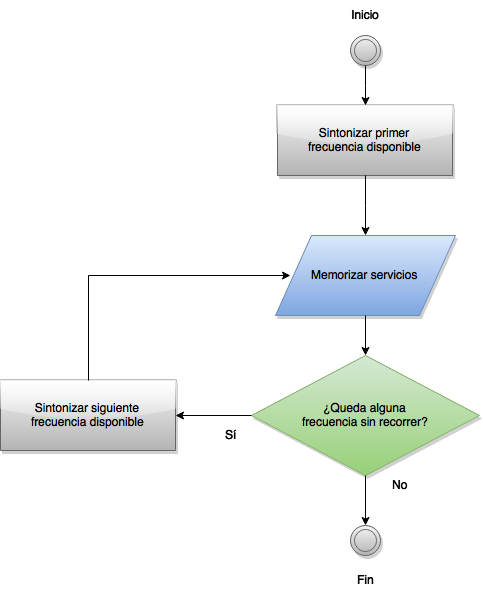
\includegraphics[width=6cm]{proceso_scan.png}
				\end{center}
				% Aclarar que scan es lo mismo que construcción de lista
				% de servicios
			\end{frame}

			\begin{frame}
				\frametitle{Recepción de señal ISDB-Tb: Sintonización}
				\begin{center}
					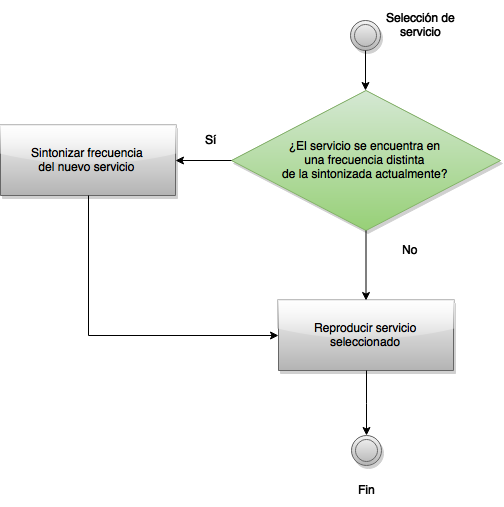
\includegraphics[width=6cm]{proceso_seleccion.png}
				\end{center}
				% Aclarar que sintonización es lo mismo que 
				% selección de servicios
			\end{frame}

			\begin{frame}
				\frametitle{Tablas en MPEG-TS}
				\begin{columns}[c] % ,t
				\column{.45\textwidth}
					\textbf{PSI:}\\
					\begin{itemize}
						\item PAT
						\item PMT
						\item \emph{NIT}
						\item \emph{CAT}
					\end{itemize}
				\column{.45\textwidth}
					\textbf{ISDB-Tb}
					\begin{itemize}
						\item SDT
					\end{itemize}
					% Recordar mencionar las secciones
			\end{columns}
			\end{frame}

			\begin{frame}
				\frametitle{Tablas en MPEG-TS}
					\begin{center}
						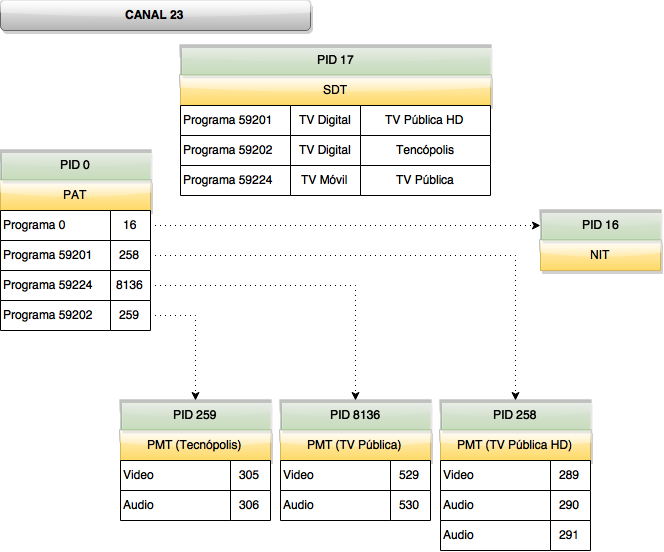
\includegraphics[width=6cm]{canal_23_tables.png}
					\end{center}
			\end{frame}

			\begin{frame}
				\frametitle{Descriptores}
				\resizebox{\textwidth}{!}{
					\lstinputlisting[]{source/dvbsnoop.txt}
				}
			\end{frame}

			\begin{frame}
				\frametitle{Flujos Elementales}
				\begin{center}
					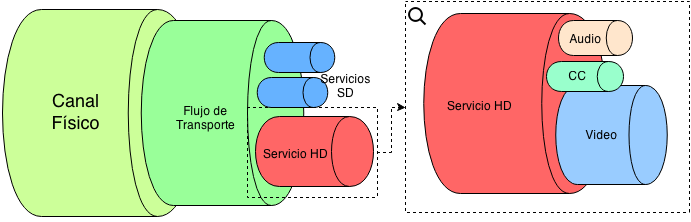
\includegraphics[width=8cm]{cable_flujo_mpeg.png}
				\end{center}
			\end{frame}
			
			\begin{frame}
				\frametitle{Decodificación de Tablas}
					\begin{center}
						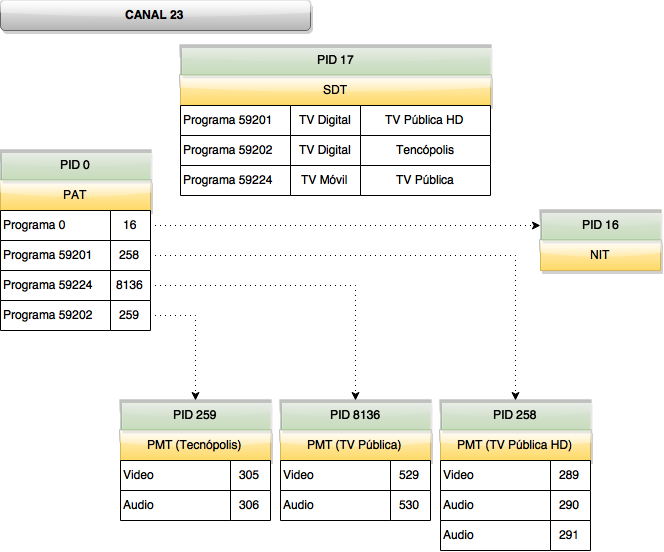
\includegraphics[width=6cm]{canal_23_tables.png}
					\end{center}
			\end{frame}

			\begin{frame}
				\frametitle{Tablas en el Scan}
					\begin{center}
						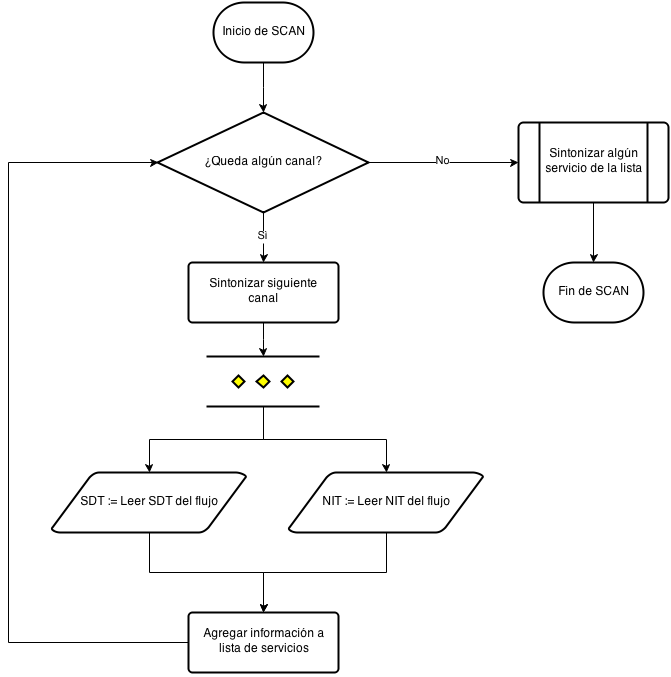
\includegraphics[width=6cm]{scan_seq_diag.png}
					\end{center}
			\end{frame}

			\begin{frame}
				\frametitle{Tablas en la sintonización}
					\begin{center}
						\includegraphics[height=6cm]{play_seq_diagram.png}
					\end{center}
			\end{frame}
			
		\subsubsection{Generación de la señal ISDB-Tb}

			\begin{frame}
				\frametitle{Generación de señal ISDB-Tb}
				\begin{itemize}
					\item Generación de contenidos
					\item Codificación y empaquetado
					\item Señalización y multiplexación de programas
				\end{itemize}
			\end{frame}

	\subsection{OpenCaster}
		\begin{frame}
			\frametitle{OpenCaster}
			\begin{columns}
			\column{.45\textwidth}
				\begin{center}
					
\includegraphics[height=3.2cm]{opencaster_logo.png}
				\end{center}
				
			\column{.45\textwidth}
					\begin{itemize}
						\item Licencia GPL
						\item Creación de entidades de normas de TV
							\begin{itemize}
								\item API para scripts Python 
							\end{itemize}
						\item Herramientas de codificación y multiplexado
					\end{itemize}
			\end{columns}
		\end{frame}

		\begin{frame}
			\frametitle{Construcción de tablas en OpenCaster}
			\resizebox{7cm}{!}{
					\lstinputlisting[language=Python]{source/pmt_example.py}
			}
		\end{frame}

	\subsection{Recepción y decodificación}
		\begin{frame}
			\frametitle{Recepción y decodificación de ISDB-Tb}
			\begin{itemize}
				\item Eventos asincrónicos
				\item \emph{Soft Real Time}
				\item Dominio intrínsecamente \emph{concurrente}
			\end{itemize}
		\end{frame}

		\subsubsection{Wari}
			\begin{frame}
				\frametitle{Wari}
				\begin{textblock*}{5cm}(7cm,1.5cm) % {block width} (coords)
					
\includegraphics[width=1.5cm]{logo_wari.png}
				\end{textblock*}
				\begin{itemize}
					\item Reproductor de TV digital terrestre
					\item Norma ISDB-Tb
					\item Licencia LGPL
					\item Desarrollado primordialmente en C++ y Lua
				\end{itemize}
			\end{frame}

			\begin{frame}
				\frametitle{Scan en Wari}
				\begin{center}
					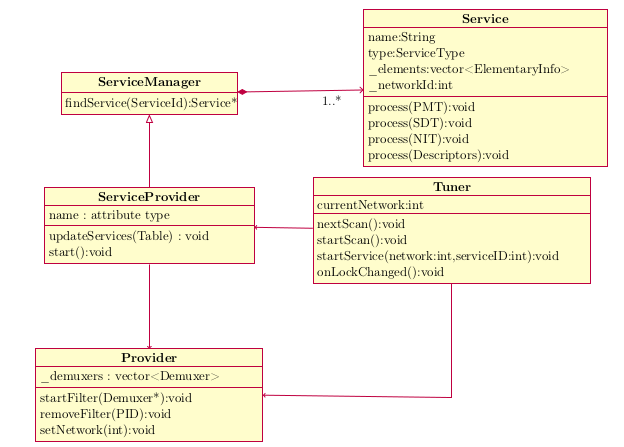
\includegraphics[width=7cm]{scan_wari.png}
				\end{center}
			\end{frame}

			\begin{frame}
				\frametitle{Sintonización en Wari}
				\begin{center}
					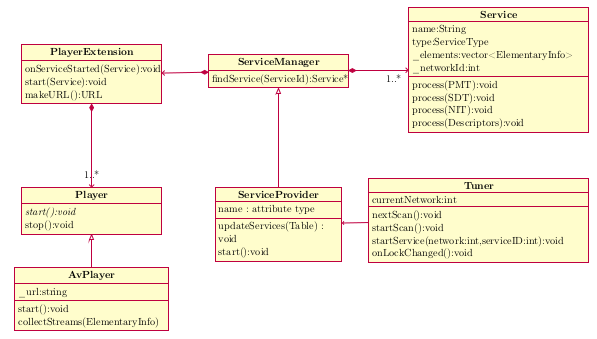
\includegraphics[width=8.5cm]{play_wari.png}
				\end{center}
			\end{frame}

	\subsection{IPTV}
		\begin{frame}
			\frametitle{IPTV}
			\begin{definition}
				Define la entrega de servicios (televisión, video, audio, texto, imágenes, datos) sobre redes basadas en IP manejadas para proveer el nivel requerido de calidad de servicio y experiencia, seguridad, interactividad y confiabilidad.
			\end{definition}
			\begin{itemize}
				\item Bitrate Variable
				\item Conmutación de paquetes
				\item \emph{Multicasting}
			\end{itemize}			
		\end{frame}

		\begin{frame}
			\frametitle{Definición de IPTV}
			\begin{definition}
			IPTV define la entrega de servicios audiovisuales en emisión \emph{multicast} a través de una red IP, donde cada servicio se limita a la multiplexación de un flujo de audio y uno de video junto con la información indispensable para la reproducción simultánea y sincronizada.
			\end{definition}			
		\end{frame}
		
		\subsubsection{Multicasting}
		\begin{frame}
			\frametitle{Multicasting}
			\begin{itemize}
				\item Requiere soporte de la infraestructura
				\item Utiliza protocolo UDP
				\item No ofrece protección ante pérdida de paquetes
				\item Rango de direcciones entre 224.0.0.0 a 239.255.255.255
				\item Los datagramas requieren un puerto destino
			\end{itemize}
		\end{frame}

\section{Diseño y Desarrollo}
\begin{frame}
%\frametitle{A first slide}

\begin{center}
\Huge Diseño y Desarrollo
\end{center}

\end{frame}
	\begin{frame}
		\frametitle{Diseño y Desarrollo}
		\begin{itemize}
			\item Señalización de servicios desde TV Terrestre hacia IPTV
			\item Construcción de un Flujo de Transporte de referencia
			\item Implementación de un sistema de emisión IPTV
			\item Desarrollo de un prototipo híbrido de recepción
		\end{itemize}
	\end{frame}


	\subsection{Señalización de los Servicios}
	\begin{frame}
		\frametitle{Primer objetivo: Señalización de servicios}
		\begin{itemize}
			\item \textbf{Centralizada:} Provista por un único medio
			\item \textbf{Transparente:} Señal emitida por cualquier medio indistintamente
			\item \textbf{Disponible para todos los dispositivos} independientemente de su acceso a la red
			\item \textbf{Uso de infraestructura existente}
		\end{itemize}
	\end{frame}

		\subsubsection{Diseño de la señalización}
		\begin{frame}
			\frametitle{Diseño de la señalización I}
				\begin{center}
					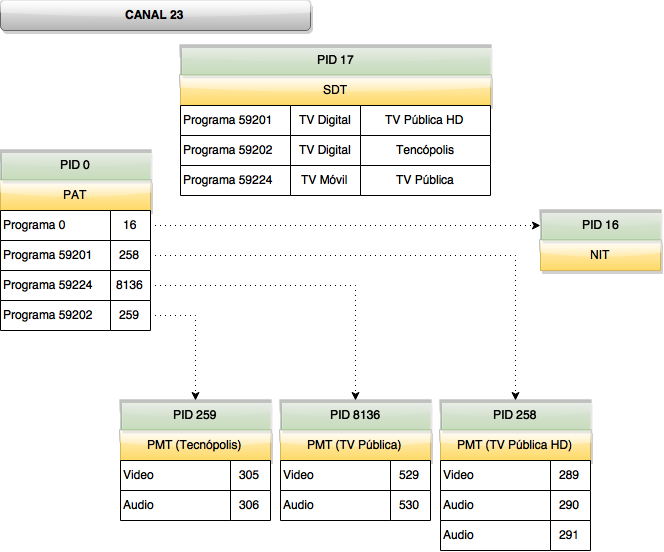
\includegraphics[width=6cm]{canal_23_tables.png}
				\end{center}
		\end{frame}

		\begin{frame}
			\frametitle{Diseño de la señalización II}
				\resizebox{0.4\textwidth}{!}{
					\lstinputlisting[]{source/pmt_syntax.txt}
				}
		\end{frame}

		\begin{frame}
			\frametitle{Diseño de la señalización III}
			\begin{center}
				\includegraphics[width=6cm]{pmt_con_descriptor.png}
			\end{center}			
		\end{frame}

		\begin{frame}
			\frametitle{\emph{Elementary Streams Relocation Descriptor}}
			\resizebox{\textwidth}{!}{
				\begin{tabular}{ | l | c | c | c | c |} 
				\hline
				Elemento & Rango de valores & Cantidad de bits & Bit de comienzo & mnemotécnico\\
				\hline 
				\hline
				\emph{descriptor\_tag}     			& 170                         & 8        		& 0 		&	\textbf{uimsbf}  \\ 
				\emph{descriptor\_length}  			& 6                           & 8        		& 8			& 	\textbf{uimsbf}  \\
				\textbf{Grupo Multicast}            & 3758096384 -- 4026531839    & 32       		& 16		&	\textbf{uimsbf}	\\
				\textbf{Puerto}                     & 1 -- 65535                  & 16      		& 48   		&	\textbf{uimsbf}  \\
				\hline 
				\end{tabular}
			}
		\end{frame}

	\subsection{Construcción del Transport Stream de referencia}
		\begin{frame}
			\frametitle{Construcción del flujo de transporte de referencia}
			\begin{enumerate}
				\item Construir tablas necesarias
				\item Reemplazar tablas existentes
				\item Insertar nueva PMT al flujo
			\end{enumerate}
		\end{frame}

		\begin{frame}
			\frametitle{TS de referencia: Construcción de entidades}
			\begin{center}
				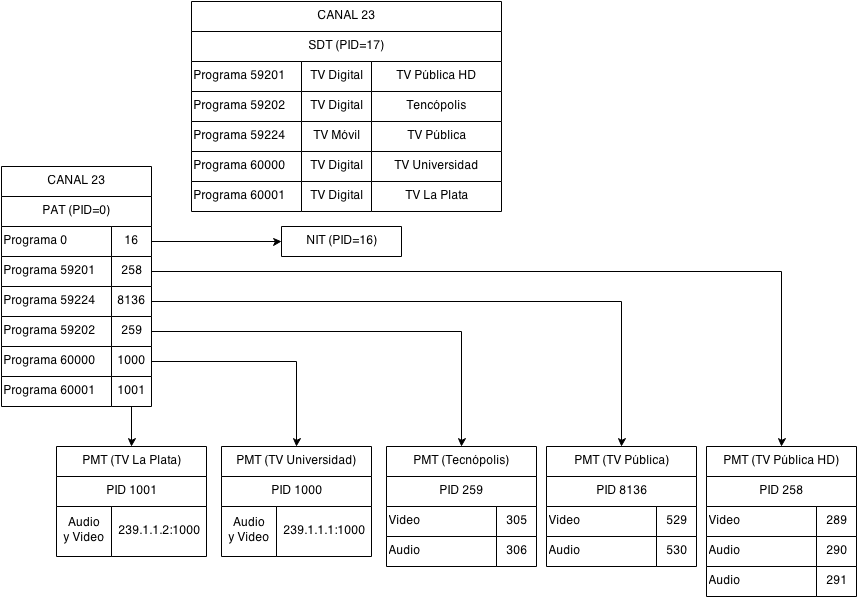
\includegraphics[width=9cm]{canal_23_extended_tables.png}
			\end{center}	
		\end{frame}

		\begin{frame}
			\frametitle{TS de referencia: Construcción de entidades II}
			\resizebox{\textwidth}{!}{
				\lstinputlisting[language=Python]{source/pmt_gen.py}
			}
		\end{frame}

		\begin{frame}
			\frametitle{TS de referencia: Multiplexación}
			\resizebox{\textwidth}{!}{
				\lstinputlisting[]{source/mux.sh}
			}
		\end{frame}

	\subsection{Emisión de los flujos elementales en Multicast}
		\begin{frame}
			\frametitle{Emisión multicast de flujos elementales}
			\begin{center}
				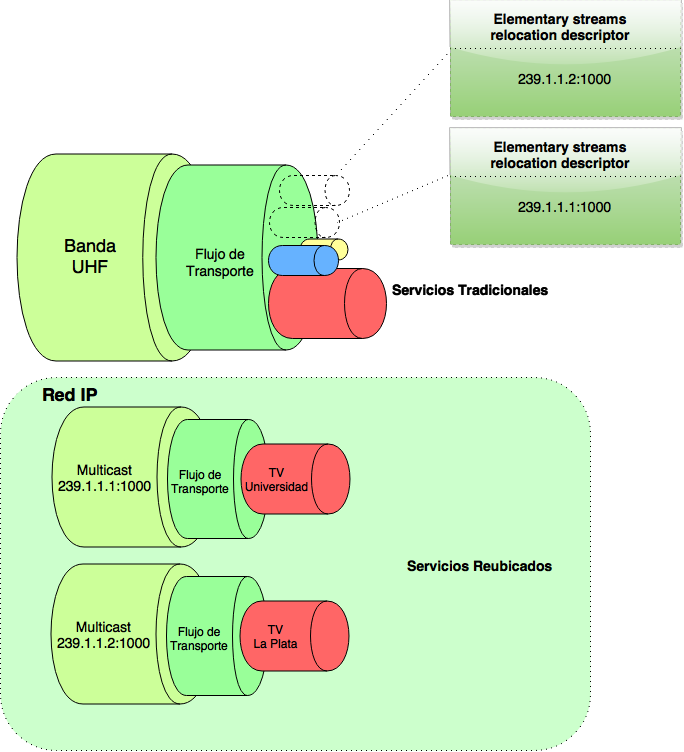
\includegraphics[width=7cm]{cable_flujo_c23e_ts.png}
			\end{center}
		\end{frame}
		
		\subsubsection{Formato Contenedor}
		\begin{frame}
			\frametitle{Formato contenedor de la emisión}
			\begin{itemize}
				\item La infraestructura existente ya ofrece soporte para MPEG-TS.
				\item Está diseñado para ambientes no confiables
				\item Es un formato extensible
				\item Provee división de paquetes adecuada a datagramas
			\end{itemize}
		\end{frame}
		
		\subsubsection{Procedimiento de emisión}
			\begin{frame}
			\frametitle{Procedimiento de emisión}
			\begin{center}
			\includegraphics[width=\textwidth]{packet_amount.png}
			$$f(t) = \frac{t[seg] * b[bits/seg]}{1504[bits/pkt]} + v[bytes] \bdiv 188[bytes/pkt] $$
			\end{center}
		\end{frame}

		\subsubsection{Procedimiento de emisión}
			\begin{frame}
			\frametitle{Procedimiento de emisión}
			\resizebox{\textwidth}{!}{
				\lstinputlisting[]{source/pseudo_streamer.txt}
			}
		\end{frame}

	\subsection{Prototipo de Recepción Mara}
		\begin{frame}
			\frametitle{Mara: Prototipo de Recepción}
			\begin{enumerate}
				\item Modificar el modelo para dar soporte a servicios reubicados
				\item Agregar un parser para el \emph{Elementary Streams Relocation Descriptor}
				\item Agregar infraestructura de reproducción de servicios reubicados
			\end{enumerate}
		\end{frame}

		% Categorías de trabajo
		\subsubsection{Modificación del modelo}
		\begin{frame}
			\frametitle{Modificación del modelo de Wari}
			\begin{center}
				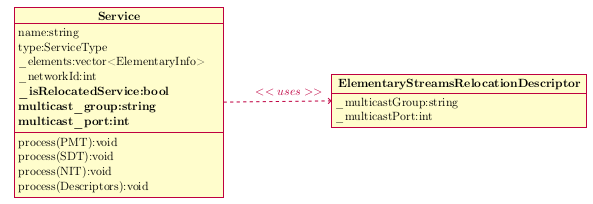
\includegraphics[width=8.5cm]{service_new_model.png}
			\end{center}
		\end{frame}

		\subsubsection{Parsing del Descriptor}
		\begin{frame}
			\frametitle{\emph{Parsing} del Elementary Stream Relocation Descriptor}
			\resizebox{\textwidth}{!}{
				\lstinputlisting[]{source/desc_parse.cpp}
			}
		\end{frame}

		\subsubsection{Reproducción de Servicios Reubicados}
		\begin{frame}
			\frametitle{Reproducción de Servicios Reubicados}
			\resizebox{\textwidth}{!}{
				\lstinputlisting[]{source/mara_play.cpp}
			}
		\end{frame}
		\begin{frame}
			\frametitle{Resultado}
			\begin{center}
				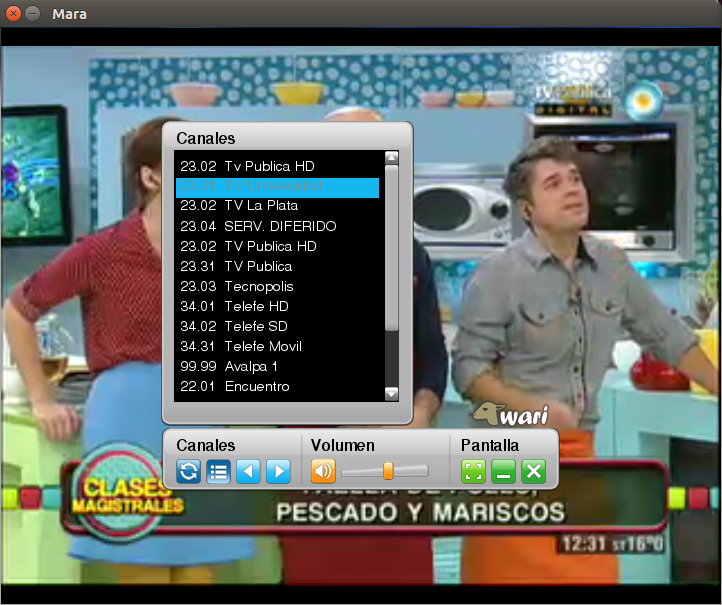
\includegraphics[width=8.5cm]{screenshot_mara.png}
			\end{center}
		\end{frame}

\section{Evaluación}
		
\begin{frame}
%\frametitle{A first slide}

\begin{center}
\Huge Evaluación
\end{center}

\end{frame}


	\begin{frame}
		\frametitle{Evaluación del trabajo realizado}
		\begin{itemize}
			\item Infraestructura
				\begin{itemize}
					\item Real
					\item De prueba
				\end{itemize}
			\item Análisis del sistema híbrido
		\end{itemize}
	\end{frame}

	\subsection{Infraestructura Requerida}
		\begin{frame}
			\frametitle{Infraestructura requerida}
			\begin{center}
				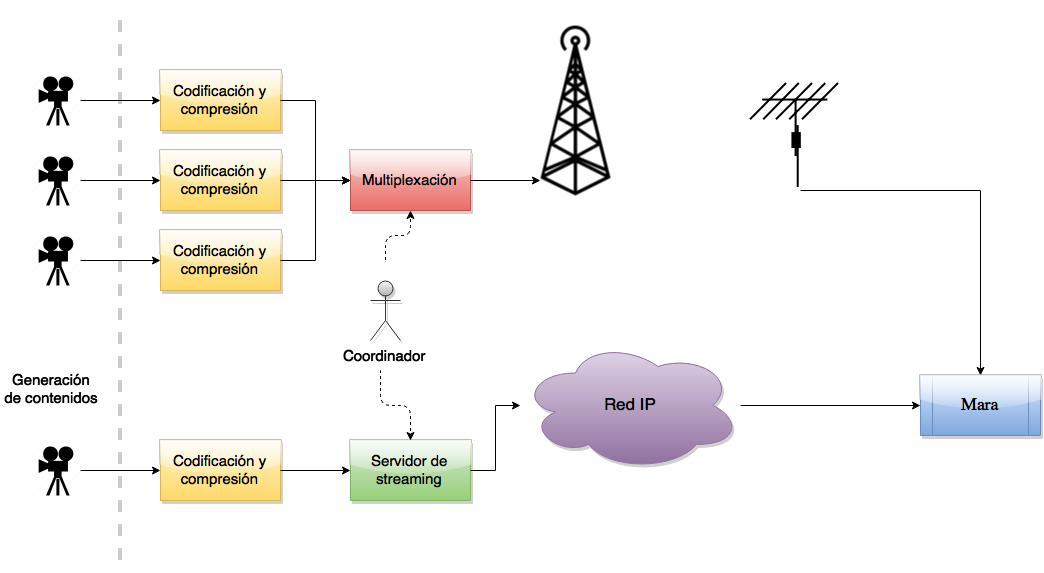
\includegraphics[width=8.5cm]{infraestructura_extendida.png}
			\end{center}
		\end{frame}

	\subsection{Infraestructura de Prueba}
		\begin{frame}
			\frametitle{Infraestructura de Prueba}
			\begin{center}
				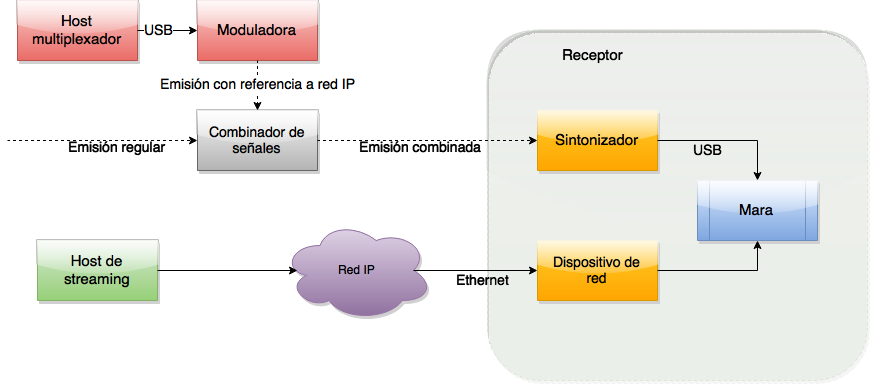
\includegraphics[width=8.5cm]{infraestructura_prueba.png}
			\end{center}
		\end{frame}

	\subsection{Análisis de la solución}
		\begin{frame}
			\frametitle{Análisis de la solución}
			\begin{center}
			\resizebox{0.6\textwidth}{!}{
			\begin{tabular}{|r|c|c|}
\hline
\rowcolor[HTML]{656565} 
{\color[HTML]{EFEFEF}Aspecto} & {\color[HTML]{EFEFEF}\begin{tabular}[c]{@{}l@{}}ISDB-Tb\\ Tradicional\end{tabular}} & {\color[HTML]{EFEFEF}ISDB-Tb + IP} \\
\hline \hline
\specialcell{Número de\\servicios} & \begin{tabular}[c]{@{}l@{}}Hasta 5 SD y\\ 1 LD\end{tabular} & Hasta 50 HD\\
\hline
\rowcolor{ashgrey}\specialcell{Múltiples Flujos\\ elementales} & \cmark & \xmark \\
\hline
\specialcell{Guía electrónica \\de programación} & \cmark & \xmark \\
\hline
\rowcolor{ashgrey}
Closed Caption & \cmark & \xmark \\
\hline
\specialcell{Gestión de\\audiencias} & \xmark & \cmark \\
\hline
\rowcolor{ashgrey}
\specialcell{Aplicaciones\\interactivas} & \cmark & \xmark \\
\hline
\specialcell{Velocidad de\\ sintonización} & 1,8s & \begin{tabular}[c]{@{}l@{}}Sintonización\\ + buffering (1,7s)\end{tabular} \\
\hline
\end{tabular}
}
\end{center}
\end{frame}



		\subsubsection{Número de servicios}
		\begin{frame}
			\frametitle{Número de servicios}
			\begin{columns}
			\column{.45\textwidth}
				\begin{itemize}
					\item \textbf{SDT:} 50 servicios
					\item \textbf{PAT:} 250 servicios
					\item \textbf{PMT:} ~200 servicios
				\end{itemize}
			\column{.45\textwidth}
				\begin{center}
					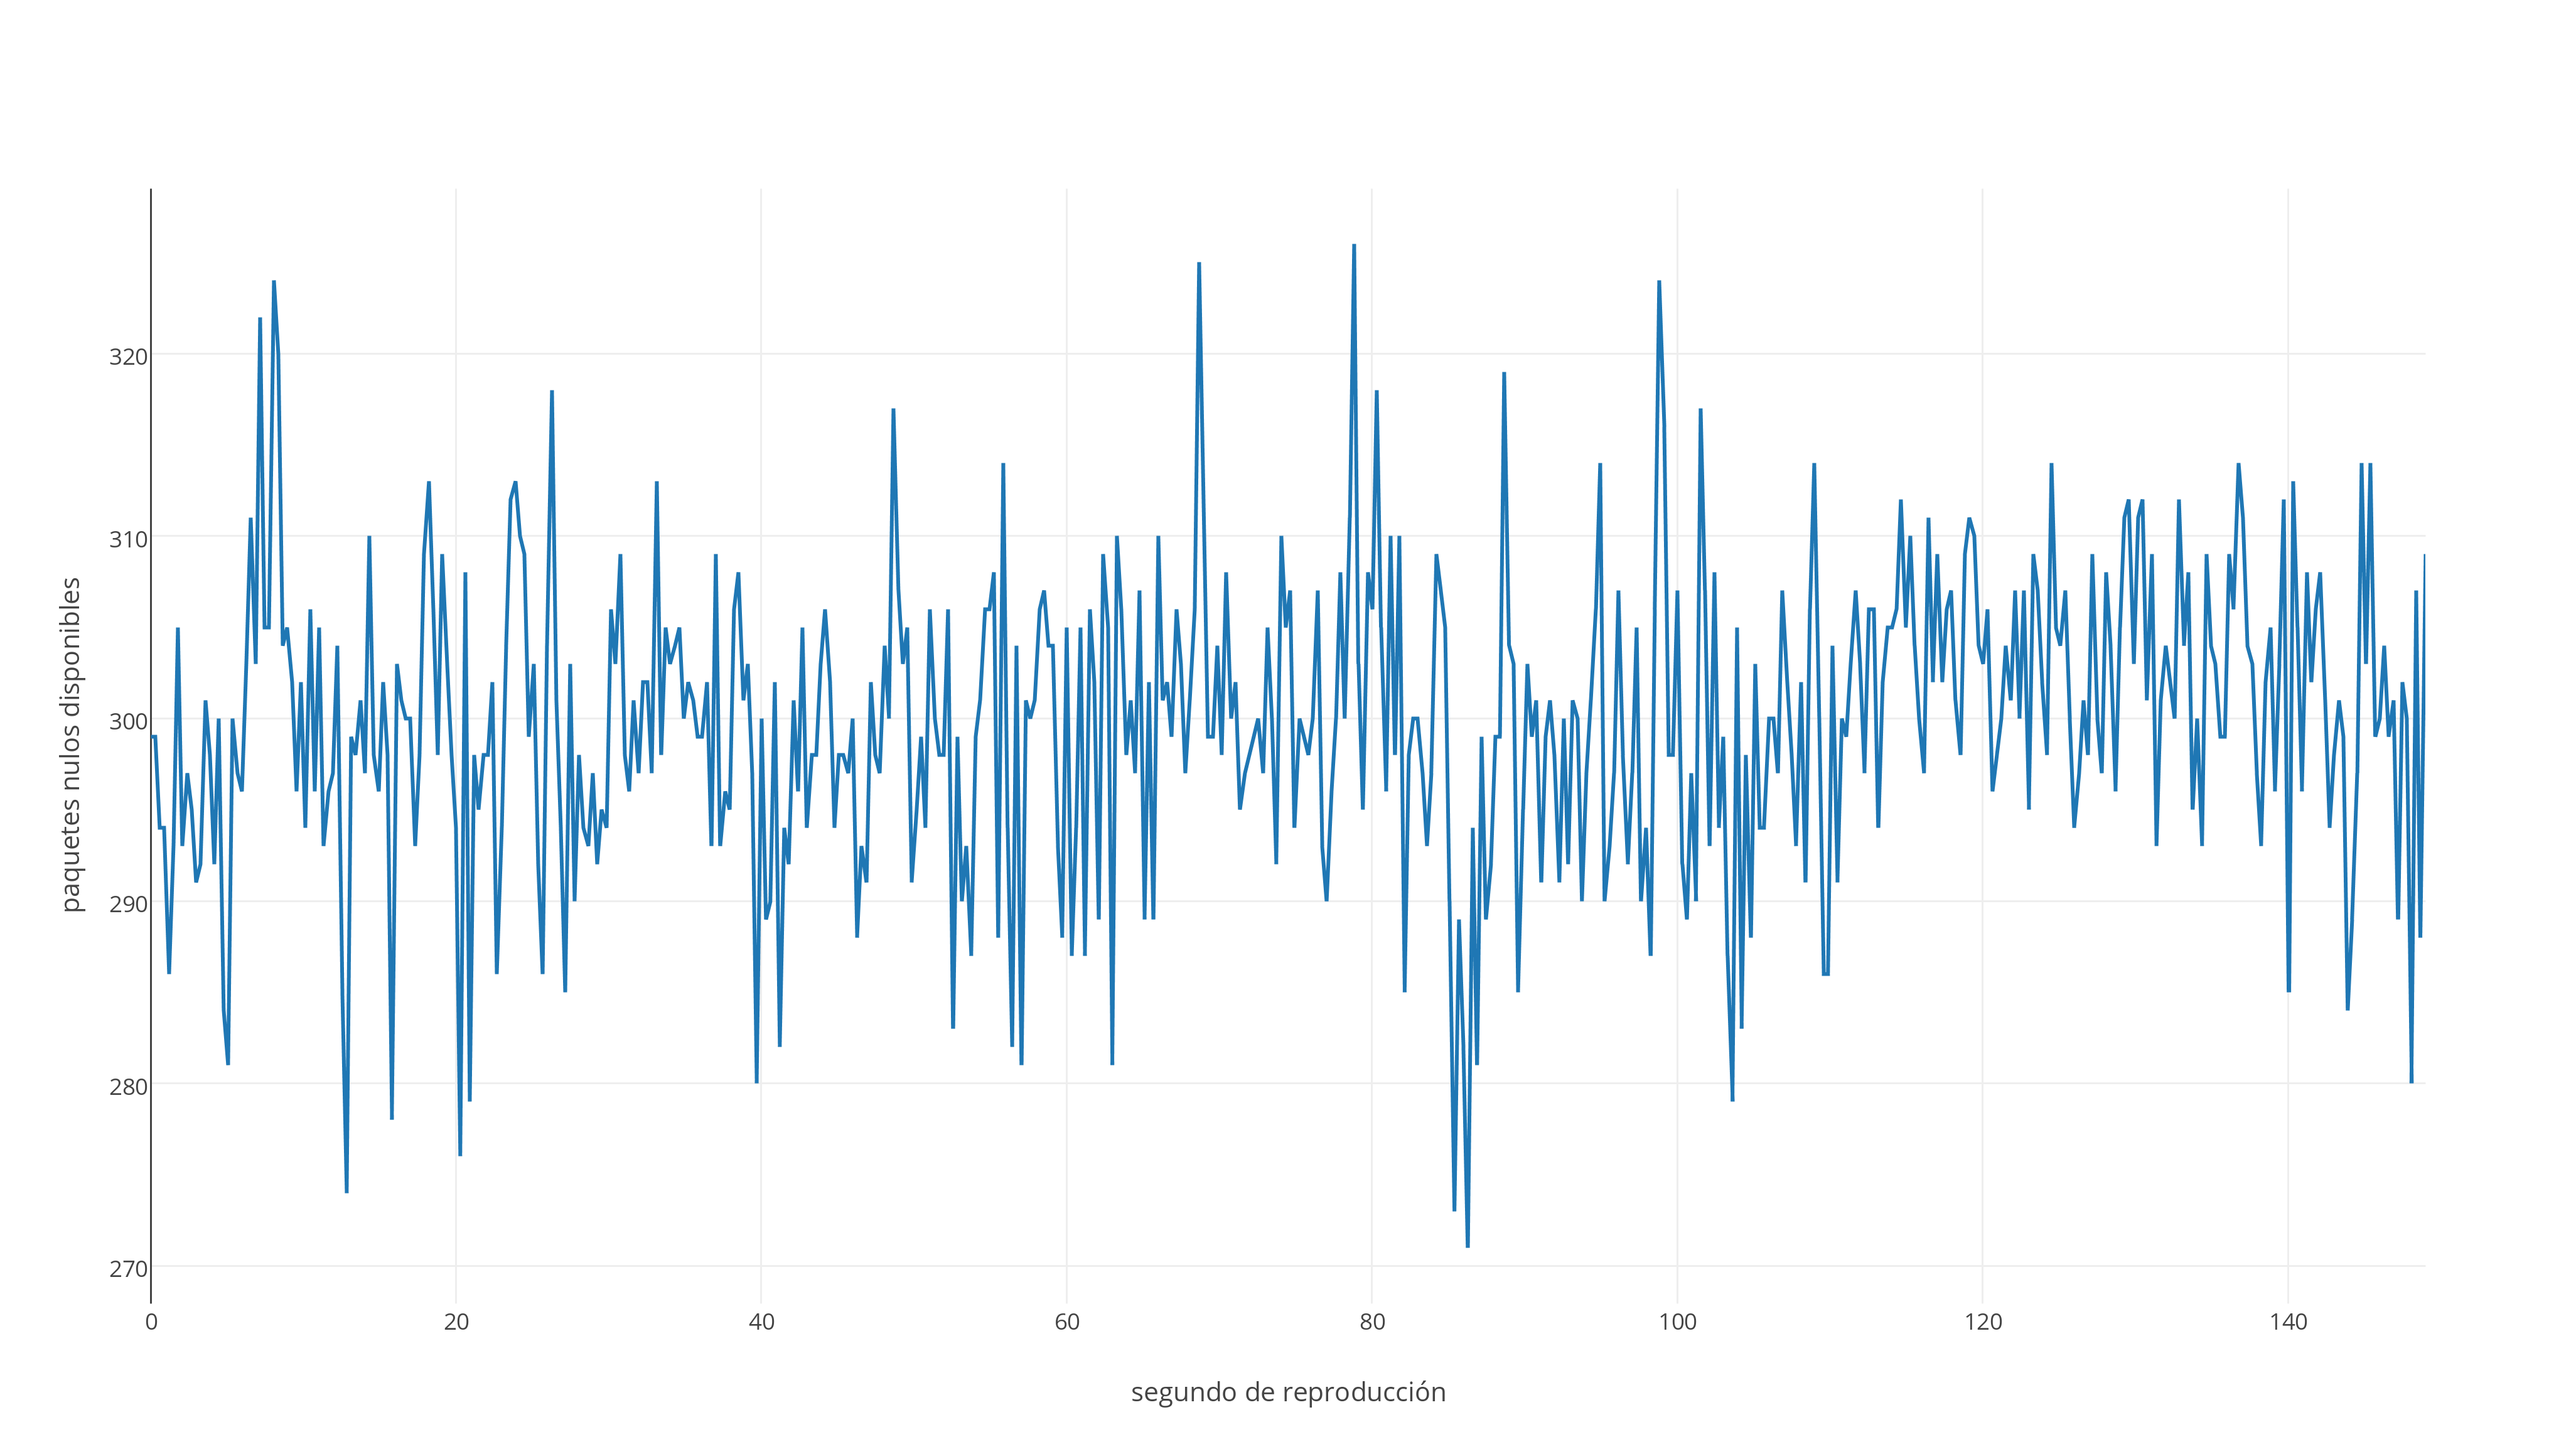
\includegraphics[width=5cm]{nulos_disponibles.png}
				\end{center}
			\end{columns}
		\end{frame}

		\subsubsection{Flujos elementales Múltiples}
		\begin{frame}
			\frametitle{Flujos elementales Múltiples}
			\begin{center}
					\includegraphics[width=9cm]{cable_flujo_mpeg_multiple_es.png}
				\end{center}
		\end{frame}

		\subsubsection{Guía Electrónica de Programación}
		\begin{frame}
			\frametitle{Guía Electrónica de Programación}
			\begin{textblock*}{5cm}(.5cm,1.5cm) % {block width} (coords)
				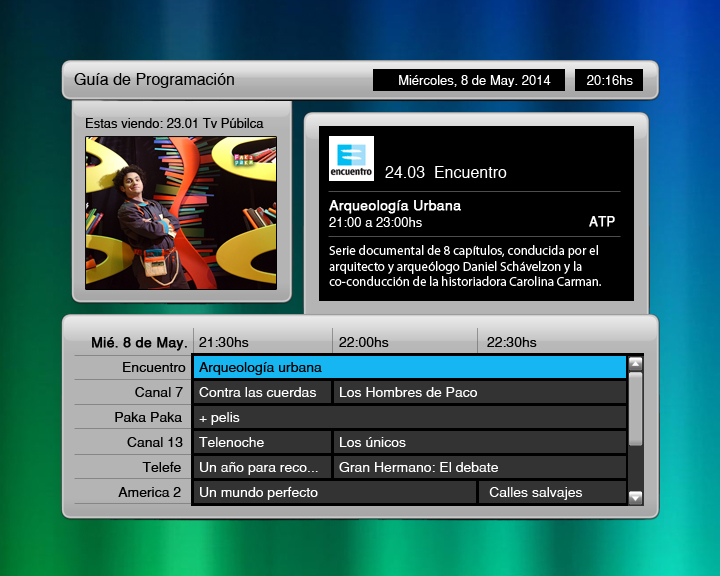
\includegraphics[width=5cm]{epg_wari.jpg}
			\end{textblock*}
			\begin{center}
			\begin{textblock*}{5cm}(6cm,5cm) % {block width} (coords)
				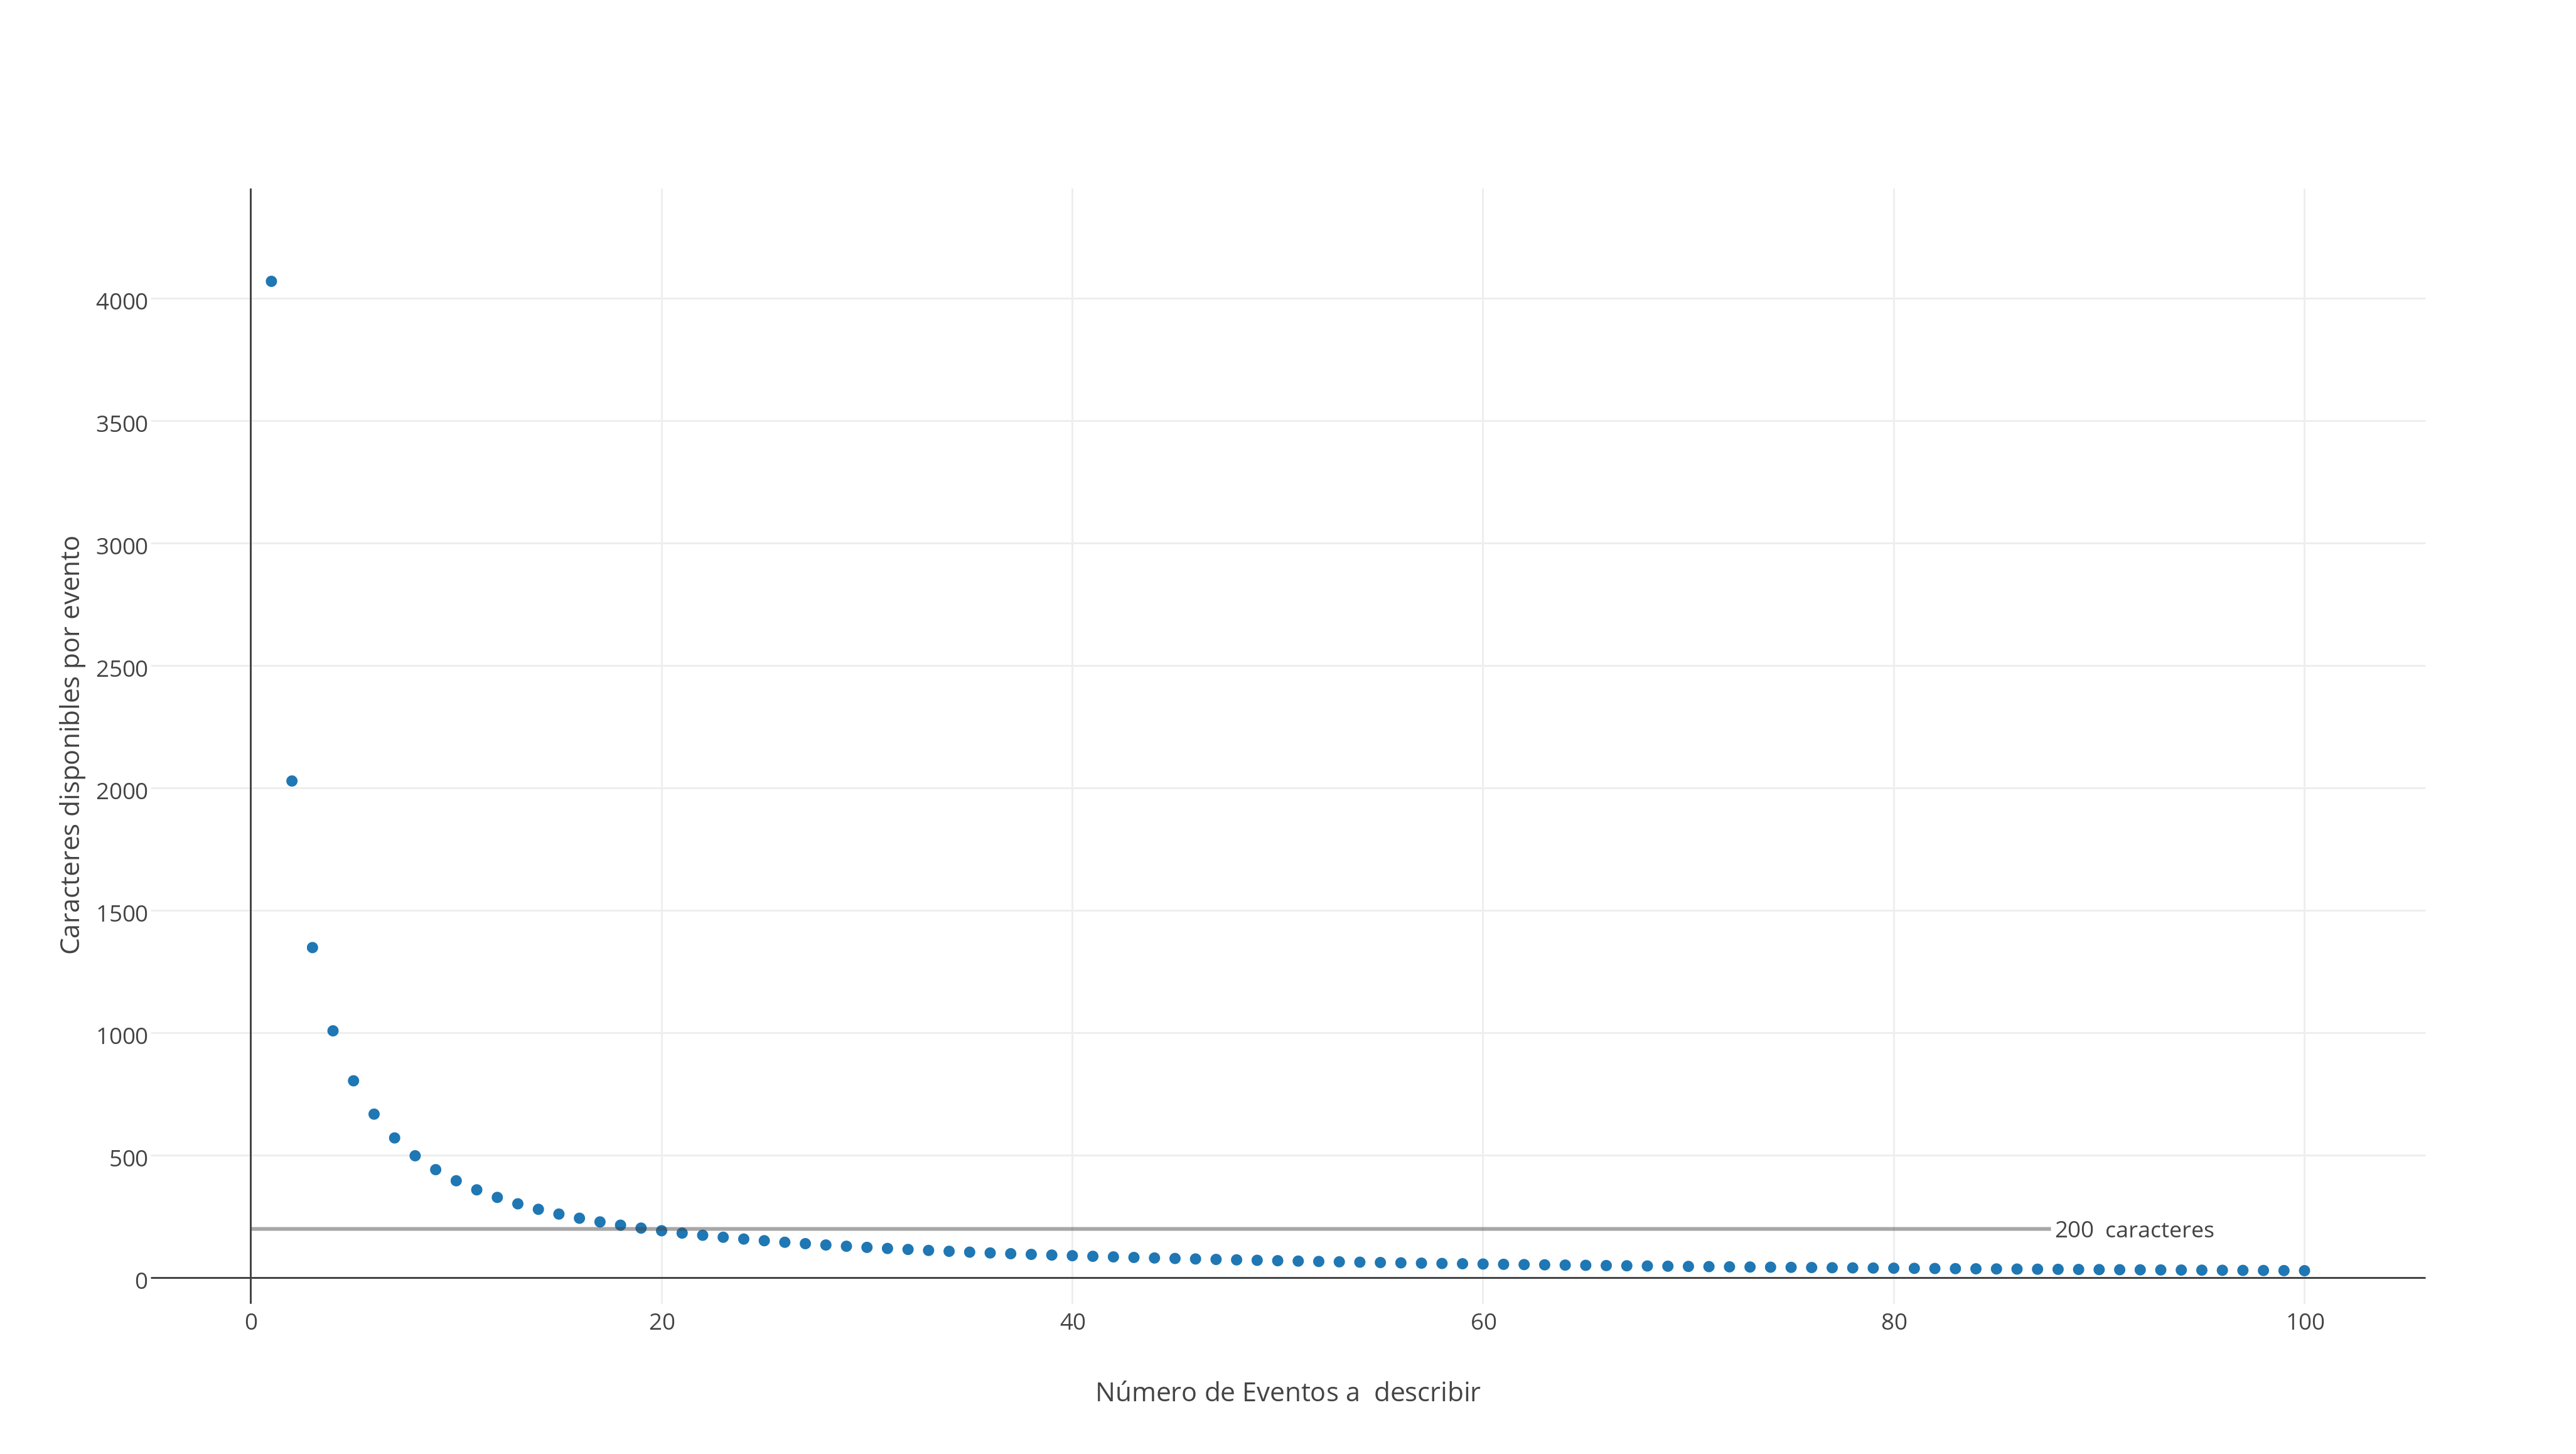
\includegraphics[width=6.5cm]{eit_size.png}
			\end{textblock*}
			\end{center}
		\end{frame}

		\subsubsection{Closed Caption}
		\begin{frame}
			\frametitle{Closed Caption}
			\begin{columns}
			\column{.45\textwidth}
				\begin{itemize}
					\item Embebidos
					\item Señalizados
				\end{itemize}
			\column{.45\textwidth}
				\begin{center}
					
\includegraphics[width=5cm]{closed_caption.jpg}
				\end{center}
			\end{columns}
			
		\end{frame}

		\subsubsection{Gestión de Audiencias}
		\begin{frame}
			\frametitle{Gestión de Audiencias}
			\begin{center}
					\includegraphics[width=8cm]{gestion_audiencias.png}
				\end{center}
		\end{frame}

		\subsubsection{Aplicaciones Interactivas}
		\begin{frame}
			\frametitle{Aplicaciones Interactivas}
			\begin{center}
					
\includegraphics[width=8cm]{sokoban.jpg}
				\end{center}
		\end{frame}

		\subsubsection{Tiempos de sintonización}
		\begin{frame}
			\frametitle{Tiempos de Sintonización}
			\begin{center}
					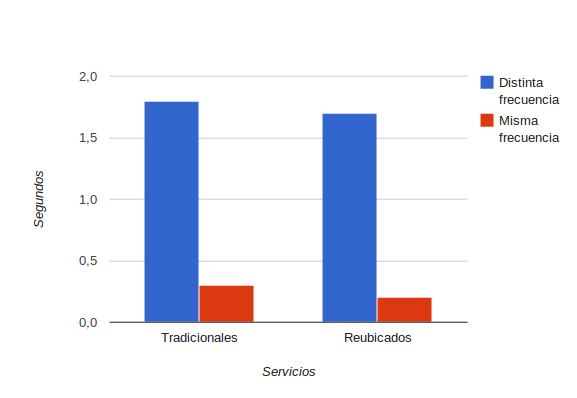
\includegraphics[width=8cm]{tune_time.png}
				\end{center}
		\end{frame}

\section{Conclusión}	

\begin{frame}
%\frametitle{A first slide}

\begin{center}
\Huge Conclusión
\end{center}

\end{frame}

	\begin{frame}
		\frametitle{Conclusión - Temario}
		\begin{itemize}
		\item Características del resultado
		\item Mara
		\item Trabajo Futuro
		\begin{itemize}
			\item Reubicación en \emph{Object Based Broadcasting}
			\item Reubicación por eventos
			\item Soporte de IPV6
			\item Omisión de PMT pequeñas
		\end{itemize}
		\item Conclusión
	\end{itemize}
	\end{frame}
	\subsection{Características del resultado}
	\begin{frame}
		\frametitle{Características del resultado}
		\begin{itemize}
		\item Mayor tamaño de la lista de servicios
		\item Retrocompatibilidad
		\item Escalable
		\item Dinámico
		\item Independiente del multiplexador
		\item Preserva bitrate
		\item Preserva dependientes
		\end{itemize}
	\end{frame}

		\subsubsection{Mara}
		\begin{frame}
			\frametitle{Prototipo de reproducción Mara}
			\begin{itemize}
			\item OpenSource
			\item Transparente
			\item Portable
			\item Independiente del Hardware
			\item No introduce dependencias tecnológicas
			\end{itemize}
		\end{frame}
	
	\subsection{Trabajo Futuro}
	\begin{frame}
		\frametitle{Trabajos futuros}
		\begin{itemize}
			\item Reubicación en Object Based Multicasting
			\item Reubicación por eventos
			\item Soporte de IPV6
			\item Omisión de PMT pequeños
		\end{itemize}
	\end{frame}
		
		\subsubsection{Reubicación en Object Based Multicasting}
		\begin{frame}
			\frametitle{Reubicación en Object Based Multicasting}
			\begin{center}
				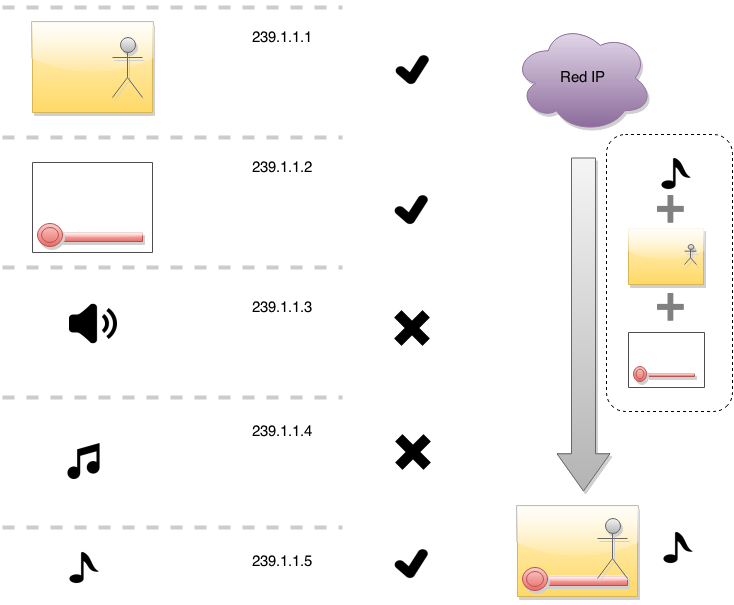
\includegraphics[width=8cm]{object_based_multicast.png}
			\end{center}
		\end{frame}

		\subsubsection{Reubicación por eventos}
		\begin{frame}
			\frametitle{Reubicación por eventos}
			\begin{center}
				\includegraphics[width=8cm]{reubicacion_eventos.png}
			\end{center}
		\end{frame}
		
		\subsubsection{Soporte de IPV6}
		\begin{frame}
			\frametitle{Soporte de IPV6}
			\resizebox{\textwidth}{!}{
				\begin{tabular}{ | l | c | c | c | c |} 
				\hline
				Elemento & Rango de valores & Cantidad de bits & Bit de comienzo & mnemotécnico\\
				\hline 
				\hline
				\emph{descriptor\_tag}     			& 170                         & 8        		& 0 		&	\textbf{uimsbf}  \\ 
				\emph{descriptor\_length}  			& 6                           & 8        		& 8			& 	\textbf{uimsbf}  \\
				\textbf{IP Version} 				& 0 -- 1 & 1 & 16 & uimsbf \\
				Reserved & -- & 7 & 17 & -- \\
				\hline
				\multicolumn{5}{| l |}{if (IP Version == 0)\{}\\
				\hline
				\textbf{Grupo Multicast}            & 3758096384 -- 4026531839    & 32       		& 24		&	\textbf{uimsbf}	\\
				\textbf{Puerto}                     & 1 -- 65535                  & 16      		& 56   		&	\textbf{uimsbf}  \\
				\hline
				\multicolumn{5}{| l |}{\} else \{ }\\
				\hline
				\textbf{Grupo Multicast}            & -- & 128 & 24		&	\textbf{uimsbf}	\\
				\textbf{Puerto}                     & 1 -- 65535                  & 16      		& 152   		&	\textbf{uimsbf}  \\
				\hline
				\multicolumn{5}{| l |}{\}}\\
				\hline 
				\end{tabular}
			}
		\end{frame}
		
		\subsubsection{Omisión de PMT Pequeñas}
		\begin{frame}
			\frametitle{Omisión de PMT Pequeñas}
			\begin{center}
				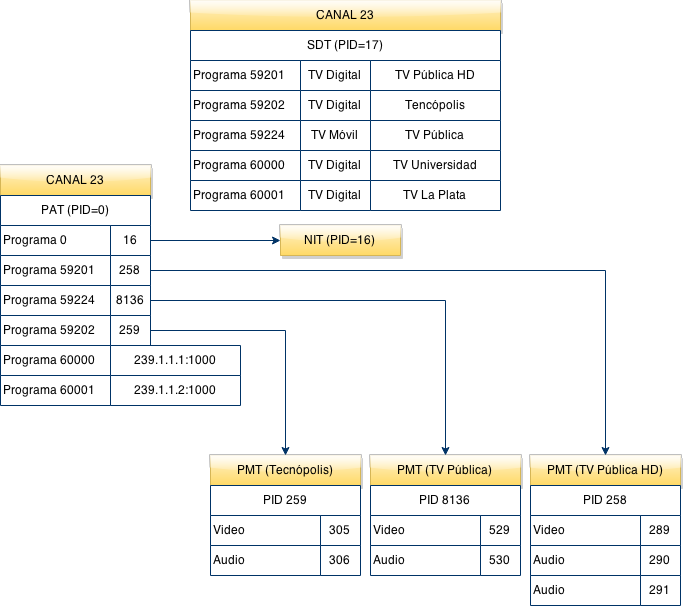
\includegraphics[width=8cm]{canal_23_no_pmt.png}
			\end{center}
		\end{frame}


	\subsection{Contribución y resultados obtenidos}
	\begin{frame}
		\frametitle{Contribución y resultados obtenidos}
		\begin{itemize}
			\item Esquema de extensión del formato MPEG-2 Transport Stream
			\item Prototipo de la transmisión de la norma ISDB-Tb extendida y construcción de flujos de transporte de referencia
			\item Prototipo de recepción del formato híbrido de transmisión ISDB-Tb e IPTV
			\item Análisis de impacto y beneficio del nuevo formato de transmisión
		\end{itemize}
	\end{frame}


\end{document} 